%!TEX program=xelatex

\documentclass[lang=cn,11pt]{elegantpaper}

\title{定义编译器功能\&汇编编程}
\author{李  科}

\institute{学号:1711344}

% 不需要版本信息,直接注释即可
%\version{0.07}
% 不需要时间信息的话,需要把 \today 删除。
\date{}


% 如果想修改参考文献样式,请把这行注释掉
%\usepackage[authoryear]{gbt7714}  % 国标
\usepackage{float}
\usepackage{url}


\begin{document}

\maketitle

\begin{abstract}
\noindent 本文主要使用上下文无关文法对C语言中常见的语法结构进行了描述。了解尝试了使用MAMS32把C语言程序(或C++)转化为汇编程序的过程。
\keywords{MAMS32,汇编,上下文无关文法}
\end{abstract}


\section{CFG描述C语言}
根据C语言的语法,C语言有37个关键字,9种控制语句,程序书写形式自由,主要用小写字母表示,压缩了一切不必要的成分。C语言不提供输入和输出语句、有关文件操作的语句和动态内存管理的语句等,这些语句都是由编译系统提供的库函数实现的。

\subsection{符号集合}
\begin{table}[H]
  \small
  \centering
  \caption{终结符符号集合}
    \begin{tabular}{l|c}
    \toprule
          含义          &       符号            \\
    \midrule
    数据类型          &    void int char bool float double long short      \\
    标识符           &     id         \\
    常量          &         number             \\
    语句             &         if else for while            \\
    算术运算       &    + - $\ast$ $\setminus$ \% $\hat{}$ ++ -- \& |  $\sim $ $\ll$  $\gg$      \\
    关系运算         &   == > < >= <= !=     \\
    逻辑运算            &       \&\& || !            \\
    其他符号         &     [ ] ( ) , ; \{ \}        \\
    函数        &     funcname        \\
    \end{tabular}%
\end{table}%

\begin{table}[H]
  \small
  \centering
  \caption{非终结符符号集合}
    \begin{tabular}{l|c}
    \toprule
          含义          &       符号            \\
    \midrule
    数据类型  &  type\\
标识符列表  &  idlist\\
数字  &  digit\\
程序主函数  &  start\\
语句  &  stmt\\
赋值语句  &  assign-expr\\
一元表达式  &  unary-expr\\
逻辑表达式  &  logical-expr\\
声明  &  decl\\
表达式  &  expr\\
参数列表  &  paralist\\
参数声明  &  paradef\\
函数声明  &  funcdef\\
    \end{tabular}%
\end{table}%


\subsection{变量声明}
\begin{equation}
  type \to int|float|double|char|short|long 
\end{equation}
\begin{equation}
  idlist \to idlist,id|id
\end{equation}
\begin{equation}
decl \to type\;idlist
\end{equation}
其中id表示标识符,type表示变量的类型,idlist代表标识符列表,decl代表声明语句。
\setcounter{equation}{0}
\subsection{赋值语句}
\begin{equation}
digit \to number\;digit 
\end{equation}
\begin{equation}
  number \to 0|1|2|3|4|5|6|7|8|9
\end{equation}
\begin{equation}
unary-expr \to digit|id
\end{equation}
\begin{equation}
  assign-expr \to unary-expre = assign-expr|logical-expr
  \end{equation}
其中num代表数字字符,digit代表数字,logical-expr为逻辑表达式,unary-expr为一元表达式,assign-expr为赋值表达式,逻辑表达式的优先级要高于赋值表达式,却低于关系表达式的比较和算术表达式的各种运算。

\setcounter{equation}{0}
\subsection{循环分支语句}
\begin{equation}
  stmt \to if(expr)stmt \; else\; stmt
\end{equation}
\begin{equation}
  stmt \to while(expr) stmt
\end{equation}
 \begin{equation}
  stmt \to for (expr;expr;expr)stmt
 \end{equation}
 其中stmt为语句,expr为表达式

\setcounter{equation}{0}
\subsection{函数定义}
\begin{equation}
  funcdef \to type \; funcname(paralist)stmt
\end{equation}
\begin{equation}
  paralist\to paralist,paradef|paradef|\varepsilon 
\end{equation}
 \begin{equation}
 paradef\to type \; id
 \end{equation}
其中paralist 代表参数列表,paradef代表参数声明,funcname代表函数名,funcdef代表函数声明语句,$\varepsilon$代表无参,type表示函数返回类型。

\setcounter{equation}{0}
\subsection{开始}
\begin{equation}
 start\to void \;main(){stmt}|int\;main(){stmt}
\end{equation}
\begin{equation}
  paralist\to paralist,paradef|paradef|\varepsilon 
\end{equation}
 \begin{equation}
 paradef\to type \; id
 \end{equation}
其中paralist 代表参数列表,paradef代表参数声明,funcname代表函数名,funcdef代表函数声明语句,$\varepsilon$代表无参,type表示函数返回类型。

\section{编写汇编程序}

\subsection{C++程序}
\begin{lstlisting}[language=C++]
  main()
  {
    int i,n,a,b,t;
    cin >> n;
    a = 0;
    i = 1;
    b = 1;
    while (i <= n)
      {
        t=b;
        b=a+b; 
        a=t;
        i=i+1;
      }
    cout<<b<<endl;
  }
\end{lstlisting}
\subsection{汇编程序}
\begin{lstlisting}[language={[x86masm]Assembler}]
 
  .486 ;告诉汇编器应该生成486处理器(或更高)的伪代码。你可以使用.386,但大多数情况下用.486
  .model flat, stdcall ;使用平坦内存模式并使用stdcall调用习惯(stdcall的意思是函数的参数从右往左压入,即最后的参数最先压入,而且函数在结束时自己清栈),这对于几乎所有的Windows API函数和dll是标准
  option casemap :none ;控制字符的映射为大写。为了Windows.inc文件能正常工作,这个应该为”none”

;为了使用来自WindowsAPI的函数,你需要导入dll。这是由导入库(.lib)来完成的。这些库是必需的。因为它们使系统(Windows)能在内存的动态基地址处动态的载入dll
  includelib \masm32\lib\kernel32.lib
  includelib \masm32\lib\user32.lib
  includelib \masm32\lib\gdi32.lib
  includelib \masm32\lib\msvcrt.lib
  includelib \masm32\lib\masm32.lib


  include \masm32\include\kernel32.inc
  include \masm32\include\user32.inc
  include \masm32\include\gdi32.inc
  include \masm32\include\windows.inc
  include \masm32\include\msvcrt.inc
  include \masm32\include\masm32.inc
  include \masm32\macros\macros.asm


     
.data  ;定义各种变量
  n dd 0;代表第几个斐波那契数
  a dd 0
  b dd 1
  i dd 1 
.code  ;写代码的地方
start:
  invoke crt_scanf,SADD("%d"),addr n;输入n
  mov ecx,i
  cmp ecx,n
  jg @2;jg为大于时跳转
@1:
  mov eax,a
  mov ebx,b
  mov a,ebx
  add ebx,eax
  mov b,ebx
  inc i
  mov ecx,i
  cmp ecx,n
  jle @1 ;i小于等于n时跳转到@1
  invoke crt_printf,SADD("%d",13,10),b ;输出结果
@2:
  ret 
   
end start
\end{lstlisting}
最后执行结果如下:

\begin{figure}[H]
\centering
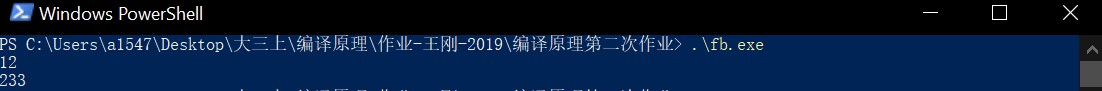
\includegraphics[width=0.8\textwidth]{result.jpg}
\caption{运行结果 \label{fig:scatter}}
\end{figure}


\section{思考:编译器如何把C程序转换为汇编程序}

\subsection{词法分析}
最开始的时候,高级语言编写的程序对编译器来说只是一连串的单个字符组成的字符串。为了让编译器识别这一连串的字符串,需要逐个字符的读取源程序,然后将其切分成有意义的单词,这些被切分后的单词在编译器眼里是以<标识,语义值>对的形式存在。
\par 为了从源程序字符串中依次找出单词,编译器需要具有扫描功能,通常这种扫描器可以用一组有限状态机来实现。
\par 我们可以用为不同类型的单词定义不同的类似的小状态机,例如变量名可以由字母、下划线组成,操作符可以取+=、->,关键字则可以是“if”“while”等单词,类型则可以是“int”“char”等等单词。为每一类单词构造一个小的有限状态机,最终组成一个可以接受不同类型单词的大状态机。可以用表的形式存放我们得到的大状态机。至此,我们通过构造一个大状态机得到一个能识别各类单词的自动扫描器。

\subsection{语法分析}
生成语法树的方法有很多,这里只介绍一种最简单的方法:预测分析法(predictive parsing)。即输入文法G,输出预测分析表M。具体做法是:从数据流的一端开始扫描,用占位符为所有之前没遇到的元素创建一个临时语法树,然后依次读取后续的数据来填充完这颗语法树。

\subsection{翻译语法树}
有了语法树后,我们接下来要做的事情是构建符号表,以便确定各个元素在存储器中的存放位置。具体做法:遍历语法树,将语法树中不同的变量依次取出,放入可用的存储位置。编译器自己决定如何分配存储位置 。语法树中多次出现的变量指向同一地址。从上到下,从左往右依次遍历语法树,遇到一个if结点,执行if相关的操作,遇到赋值结点,执行赋值相关的操作。
\par 编译器想要翻译所有的C语言程序,重要的是要知道所有的C语言的语法规则,掌握语言特性,对于每个语言特性都可以进行分类处理,即用有限的递归出无限。



\nocite{*}
\bibliographystyle{aer}
\bibliography{wpref}
\end{document}
